\newpage
\section*{11\quad Designing your own transformer}
\addcontentsline{toc}{section}{11 Designing your own transformer}
\startchapter{11}
\providecommand{\nElevenFit}[1]{\setbox0\hbox{#1}\ifdim\wd0>\linewidth\resizebox{\linewidth}{!}{\usebox0}\else\usebox0\fi}

\begin{chaptermap}
Ten chapters took one model apart. This one puts a model together from nothing, and the hard part is no
longer the mechanism but the choices. \textbf{The problem:} you have a budget (of compute, of memory, of
time) and a job. \textbf{The steps:} name every decision (\S11.1); price the three budgets, compute
(\S11.2), parameters (\S11.3) and running memory (\S11.5); see what heads and key--value sharing really
buy (\S11.4); look at what our own experiments showed and what they could not show (\S11.6); then make
one complete design and defend every line (\S11.7). \textbf{Where it ends:} a table of trade-offs you can
reuse (\S11.8), and a look back over the whole notes.
\end{chaptermap}

\machine{11}{The whole machine, built. Designing is setting its dials, and every dial sits on one block: the
vocabulary $V$ on the token and embedding blocks (and the scores at the bottom); the width $d$ on every arrow
of the stream; the depth $L$ on the frame, which is repeated $L$ times; the query heads $h$ and the key--value
heads inside attention; the MLP width $d_{ff}$ inside the MLP; and the context length on the KV cache at the
side, which grows with every token.}

\begin{beforeyoustart}
\begin{enumerate}[label=\arabic*.,leftmargin=1.6em]
\item How many zeros are in one billion? \emph{Refresher: thousand $=10^3$, million $=10^6$,
billion $=10^9$, trillion $=10^{12}$.}
\item What is $10^{3}\times10^{6}$? \emph{Refresher: multiplying powers of ten adds the exponents, so it
is $10^{9}$.}
\item What is $\sqrt{10^{18}}$? \emph{Refresher: a square root halves the exponent: $10^{9}$.}
\item A file is 2{,}000{,}000{,}000 bytes. How many gigabytes (GB) is that? \emph{Refresher: here
1 GB $=10^9$ bytes, so 2 GB.}
\item If a cost grows ``as the square of the width'', what happens to it when the width doubles?
\emph{Refresher: $2^2=4$, so it becomes four times bigger.}
\end{enumerate}
\end{beforeyoustart}

%=====================================================================
\subsection*{11.1\quad Design is a list of decisions}

Suppose someone hands you a budget and asks you to build a model. How many attention heads should it have?
How wide should the MLP be: 192? 256? How many blocks? How many numbers should describe each token, and how
would you even decide? Those questions are the whole of this chapter. Every one of those questions is a \emph{decision}, and a
decision is only as good as the \emph{assumptions} under it and the \emph{trade-off} it accepts.

\Predict Before reading on, write down every number you would have to choose to build a model like the
one in Chapter 10. How many did you get? Most people find five or six. There are about ten.

\Picture You are building a house with a fixed amount of money. You choose how wide the rooms are, how
many floors to stack, how many doors each room has, how big the storage cupboard is, and how many guests
it must hold at once. Every extra metre in one place is a metre you cannot spend somewhere else.

\Exactly A decoder-only transformer is fixed by these choices:
\begin{center}
\small
\begin{tabular}{@{}l l l@{}}
\toprule
Decision & Symbol & Where you met it\\
\midrule
vocabulary size & $V$ & Chapter 2\\
width (numbers per token) & $d$ & Chapters 2, 3\\
depth (number of blocks) & $L$ & Chapters 5, 6\\
query heads and head size & $H$, $d_h$ with $H d_h = d$ & Chapters 3, 5\\
key--value heads & $H_{kv}$ & Chapter 9\\
MLP width and type & $d_{ff}$, GELU or SwiGLU & Chapter 5\\
normalisation and where it sits & LayerNorm or RMSNorm, before or after & Chapter 6\\
positional scheme & learned, sinusoid, RoPE & Chapter 4\\
context length & $n_{ctx}$ & Chapters 4, 9\\
training tokens & $D$ & Chapter 8\\
\bottomrule
\end{tabular}
\end{center}

\begin{breaks}
A house's rooms do not talk to each other. In a transformer the choices interact: the head size is the
width divided by the number of heads, and the memory needed at run time depends on depth, key--value heads
and context together. The picture gives you the budget; it does not give you the interactions.
\end{breaks}

\Why There is no formula that outputs ``the best transformer''. There are budgets, and every budget
turns some of these choices into consequences you can calculate. So the method of this chapter is
always the same: state the assumption, compute the consequence, then decide.

\Summary{Designing a transformer means fixing about ten numbers, each one a decision whose cost you can
calculate before you train anything.}

%=====================================================================
\subsection*{11.2\quad Budget 1: compute}

\Predict You double the number of parameters and also double the amount of training text. How much more
compute do you need: twice as much, three times, or four times?

\Picture Every token of training text has to pass through every weight. Think of a factory where each
item visits each machine: the work is (number of items) $\times$ (number of machines). Double both and
the work is four times larger.

\Exactly A weight touched by a token costs one multiply and one add, so two operations (FLOPs) on the
way forward. Learning needs a backward pass that costs about twice the forward one (Chapter 8). So
training costs about $2+4=6$ FLOPs per parameter per token (Kaplan et al., 2020):
\[
C \;\approx\; 6\,N\,D \qquad
\begin{array}{l}\scriptstyle C:\ \text{training FLOPs},\quad N:\ \text{parameters},\quad D:\ \text{training tokens}\end{array}
\]
So the answer to the prediction is four times. The formula ignores the attention scores themselves,
which add a little for long contexts (Chapter 10 counts them).

\paragraph{How to split a compute budget between $N$ and $D$.} If $C$ is fixed, a bigger model sees less
text and a smaller model sees more. Hoffmann et al.\ (2022) trained hundreds of models and found that,
to reach the lowest loss for a fixed $C$, parameters and tokens should grow together, with roughly
\emph{20 training tokens per parameter}. Put $D=20N$ into $C=6ND$:
\[
C = 120\,N^2 \quad\Longrightarrow\quad N_{\text{opt}} \approx \sqrt{C/120}, \qquad D_{\text{opt}} \approx 20\,N_{\text{opt}}.
\]

\paragraph{Worked example A: one CPU thread for one hour.} Our ablation models in \S11.6 have
\nElevenAbParams\ parameters and each saw \nElevenAbTokens\ tokens in about \nElevenAbSeconds\ seconds
on one thread of our build machine. That is about $\nElevenCpuFlops$ training FLOPs per second, so one
hour gives $C\approx\nElevenCpuHourFlops$. The rule of thumb then says: about \nElevenCpuNopt\
parameters trained on \nElevenCpuDopt\ tokens. Our ablation models used \nElevenAbTokPerParam\ tokens per
parameter, close to the rule.

\paragraph{Worked example B: 1{,}000 hours of a data-centre GPU.} Let's assume a GPU whose data sheet
promises \nElevenGpuPeak\ trillion FLOPs per second (NVIDIA's figure for the H100 at 16-bit precision),
and let's assume your code keeps it \nElevenGpuMfu\% busy, a common real-world figure. Then
$C\approx\nElevenGpuC$, and the rule of thumb gives about \nElevenGpuNopt\ parameters trained on
\nElevenGpuDopt\ tokens. We design that model in \S11.7.

\begin{wrongidea}{11.3}
\emph{``Compute depends on the number of parameters.''} It depends on parameters \emph{and} tokens, in
equal measure. A 1-billion-parameter model trained on a thousand times more text costs a thousand times
more.
\end{wrongidea}

\begin{wrongidea}{11.2}
\emph{``Bigger is always better.''} At a fixed compute budget, a model that is too big for its data ends
up worse than a smaller one trained on more text. That is the finding of Hoffmann et al.\ (2022): many
earlier large models were under-trained for their size.
\end{wrongidea}

\paragraph{Why modern small models ignore the 20-to-1 rule.} Qwen3-0.6B has \nElevenQwenParams\
parameters. The rule of thumb would train it on about \nElevenQwenChinTokens\ tokens. The Qwen3
technical report (2025) says the family was pre-trained on about 36 trillion tokens: roughly
\nElevenQwenTokPerParam\ tokens per parameter, a few thousand times the rule. Is that a mistake? Ask what
the rule minimises: \emph{training} compute for a given loss. But a small model is trained once and then
run billions of times. Every extra token of training makes the model better without making it bigger,
and a smaller model is cheaper on every single request forever after. When serving costs dominate, you
pay more at training time to save at run time. (We take the 36-trillion figure from the report and could
not check it ourselves.)

\begin{breaks}
The factory picture says the cost is items times machines. It does not say whether more items or more
machines gives a better product; that question needed experiments (Hoffmann et al.), and the answer
changes once you count what the product costs to use.
\end{breaks}

\Why Compute is the one budget you cannot borrow against. Writing $C\approx6ND$ first turns a vague wish
(``a good model'') into two numbers you can argue about.

\begin{checkq}
You have a fixed compute budget and you decide to make the model 4 times bigger. By the rule of thumb in
this section, what should happen to the number of training tokens?
\begin{options}
\item Stay the same; compute only depends on parameters.
\item Shrink to a quarter, since $C=6ND$ is fixed.
\item The plan breaks the 20-to-1 balance; with $C$ fixed you should not grow $N$ alone.
\item Grow 4 times, because bigger models always need more data, whatever the budget.
\end{options}
\end{checkq}

\Summary{Training compute is about $6ND$, and for a fixed budget the loss-optimal split is roughly 20
tokens per parameter, unless running the model will cost more than training it.}

%=====================================================================
\subsection*{11.3\quad Budget 2: parameters, and where they live}

\Predict In Qwen3-0.6B, which part holds more parameters in each block: the attention or the MLP? And
what fraction of the whole model do you think is the vocabulary table?

\Picture A recipe card has one number for each ingredient. In Chapter 3 a $d\times d_k$ matrix was $d_k$
recipe cards with $d$ ingredients each. So a matrix costs (inputs) $\times$ (outputs) numbers, and
every design choice is a choice of how many cards, with how many ingredients.

\Exactly Count one block of a model with width $d$, $H$ query heads and $H_{kv}$ key--value heads of size
$d_h$, and an MLP of width $d_{ff}$:
\[
\underbrace{d\,H d_h}_{W_Q} + \underbrace{2\,d\,H_{kv} d_h}_{W_K,\,W_V} + \underbrace{H d_h\, d}_{W_O}
\;+\; \underbrace{3\,d\,d_{ff}}_{\text{SwiGLU MLP}} \;+\; \text{(small norm vectors)}.
\]
The model adds the vocabulary table $V d$ (and a second one if the output layer is not tied to it,
Chapter 7). For Qwen3-0.6B this gives \nElevenQwenAttn\ attention parameters and \nElevenQwenMlp\ MLP
parameters per block: the MLP is \nElevenQwenMlpShare\% of each block. The vocabulary table alone is
\nElevenQwenEmbShare\% of the whole model; in GPT-2 the token and position tables are \nElevenGptEmbShare\%.

\begin{figure}[!htb]
\centering
% AUTO-GENERATED by code/ch11_figs.py
\nElevenFit{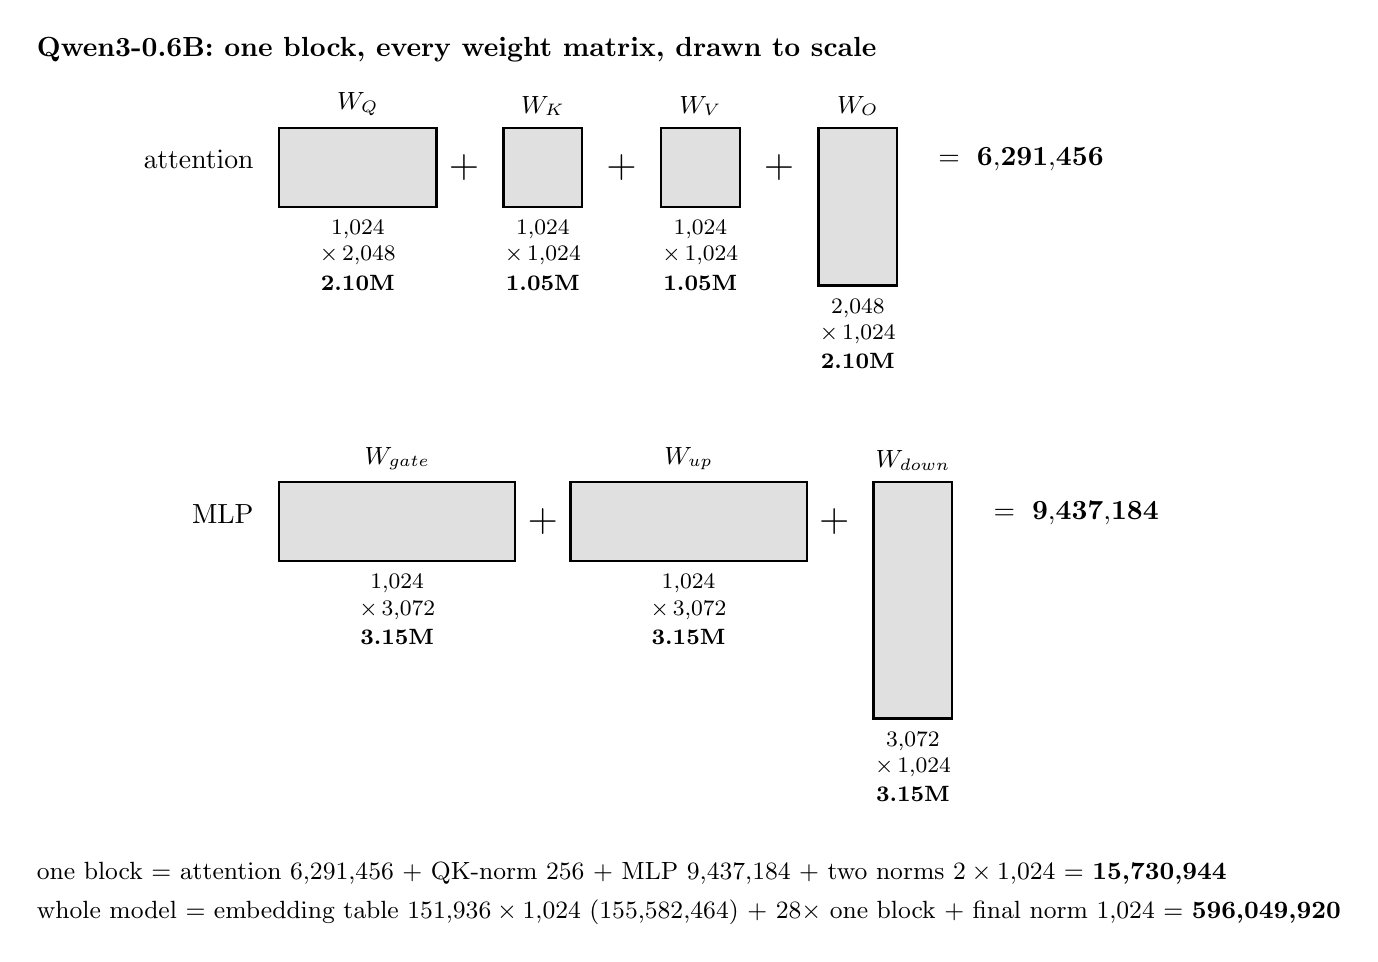
\begin{tikzpicture}
\node[anchor=west, font=\normalsize\bfseries] at (-3.2,1.0) {Qwen3-0.6B: one block, every weight matrix, drawn to scale};
\node[anchor=east, font=\normalsize, align=right] at (-0.200,-0.400) {attention};
\draw[line width=0.8pt, fill=black!12] (0.000,0.000) rectangle (2.000,-1.000);
\node[anchor=south, font=\small] at (1.000,0.030) {$W_Q$};
\node[anchor=north, font=\footnotesize, align=center] at (1.000,-1.050) {1{,}024\\$\times$\,2{,}048\\[1pt]\textbf{2.10M}};
\node[font=\Large] at (2.350,-0.500) {$+$};
\draw[line width=0.8pt, fill=black!12] (2.850,0.000) rectangle (3.850,-1.000);
\node[anchor=south, font=\small] at (3.350,0.030) {$W_K$};
\node[anchor=north, font=\footnotesize, align=center] at (3.350,-1.050) {1{,}024\\$\times$\,1{,}024\\[1pt]\textbf{1.05M}};
\node[font=\Large] at (4.350,-0.500) {$+$};
\draw[line width=0.8pt, fill=black!12] (4.850,0.000) rectangle (5.850,-1.000);
\node[anchor=south, font=\small] at (5.350,0.030) {$W_V$};
\node[anchor=north, font=\footnotesize, align=center] at (5.350,-1.050) {1{,}024\\$\times$\,1{,}024\\[1pt]\textbf{1.05M}};
\node[font=\Large] at (6.350,-0.500) {$+$};
\draw[line width=0.8pt, fill=black!12] (6.850,0.000) rectangle (7.850,-2.000);
\node[anchor=south, font=\small] at (7.350,0.030) {$W_O$};
\node[anchor=north, font=\footnotesize, align=center] at (7.350,-2.050) {2{,}048\\$\times$\,1{,}024\\[1pt]\textbf{2.10M}};
\node[anchor=west, font=\normalsize] at (8.250,-0.400) {$=\ \mathbf{6{,}291{,}456}$};
\node[anchor=east, font=\normalsize, align=right] at (-0.200,-4.900) {MLP};
\draw[line width=0.8pt, fill=black!12] (0.000,-4.500) rectangle (3.000,-5.500);
\node[anchor=south, font=\small] at (1.500,-4.470) {$W_{\text{gate}}$};
\node[anchor=north, font=\footnotesize, align=center] at (1.500,-5.550) {1{,}024\\$\times$\,3{,}072\\[1pt]\textbf{3.15M}};
\node[font=\Large] at (3.350,-5.000) {$+$};
\draw[line width=0.8pt, fill=black!12] (3.700,-4.500) rectangle (6.700,-5.500);
\node[anchor=south, font=\small] at (5.200,-4.470) {$W_{\text{up}}$};
\node[anchor=north, font=\footnotesize, align=center] at (5.200,-5.550) {1{,}024\\$\times$\,3{,}072\\[1pt]\textbf{3.15M}};
\node[font=\Large] at (7.050,-5.000) {$+$};
\draw[line width=0.8pt, fill=black!12] (7.550,-4.500) rectangle (8.550,-7.500);
\node[anchor=south, font=\small] at (8.050,-4.470) {$W_{\text{down}}$};
\node[anchor=north, font=\footnotesize, align=center] at (8.050,-7.550) {3{,}072\\$\times$\,1{,}024\\[1pt]\textbf{3.15M}};
\node[anchor=west, font=\normalsize] at (8.950,-4.900) {$=\ \mathbf{9{,}437{,}184}$};
\node[anchor=north west, font=\small, align=left] at (-3.2,-9.200) {one block $=$ attention 6{,}291{,}456 $+$ QK-norm 256 $+$ MLP 9{,}437{,}184 $+$ two norms $2\times1{,}024$ $=$ \textbf{15{,}730{,}944}\\[3pt]whole model $=$ embedding table $151{,}936\times1{,}024$ (155{,}582{,}464) $+\ 28\times$ one block $+$ final norm 1{,}024 $=$ \textbf{596{,}049{,}920}};
\end{tikzpicture}}

\caption{The formula above, drawn. Each rectangle is one weight matrix of a Qwen3-0.6B block, with one row per
input and one column per output, so its area is its parameter count. Add the rectangles and you get the
block; multiply by 28 and add the embedding table and you get the model. Compare the area of the MLP row with
the attention row before reading the numbers.}
\end{figure}

\Sanity Our calculator is checked two ways. Building the real Hugging Face model classes on an empty
(``meta'') device, with no weights downloaded, gives exactly \nElevenGptParams\ parameters for GPT-2 and
\nElevenQwenParams\ for Qwen3-0.6B, the same as our formula. A second calculator written for Chapter 10
gives the same totals: the check says it \nElevenCalcCheck.

\paragraph{Width versus depth.} Doubling the width $d$ multiplies every matrix in every block by about
four (both sides of each matrix grow). Doubling the depth $L$ only doubles the block count. So width is
the expensive direction for parameters, depth the expensive direction for \emph{time}: blocks run one after
another, so a deep model is slower per token even at equal size. Kaplan et al.\ (2020) found that, at a
fixed parameter count, loss depends only weakly on the exact shape across a wide range. In practice
designers keep $d/L$ somewhere between about 50 and 150 and spend their attention elsewhere.

\begin{wrongidea}{11.7}
\emph{``Width is free: a wider vector holds more information.''} It is tempting because a wider vector
can hold more. But every weight matrix in a block is $d$ by something proportional to $d$, so doubling
the width roughly quadruples the parameters and the arithmetic. Width costs quadratically.
\end{wrongidea}

\paragraph{Vocabulary size.} A bigger vocabulary means a bigger table ($Vd$ numbers) but shorter
sequences, since each token covers more text (Chapter 2). Shorter sequences make attention and the KV
cache cheaper. For a small model the table is a large share of the budget (\nElevenQwenEmbShare\% here),
which is one reason small models tie their input and output tables.

\begin{wrongidea}{11.5}
\emph{``The vocabulary is free; it is only a lookup.''} The lookup costs no FLOPs, but it costs
parameters, memory and, at the output end, a full $d\times V$ multiplication for every generated token.
\end{wrongidea}

\begin{checkq}
You double the width $d$ of a model and keep everything else in proportion ($d_{ff}=3d$, $d_h$ fixed).
Roughly what happens to the parameters inside the blocks?
\begin{options}
\item They double, like the width.
\item They grow about four times.
\item They stay the same; width only changes how tokens are described.
\item They halve, because each head gets smaller.
\end{options}
\end{checkq}

\Summary{A matrix costs inputs times outputs, so width costs quadratically, depth linearly, and the
vocabulary table can be a quarter of a small model.}

%=====================================================================
\subsection*{11.4\quad Heads, head size, and sharing keys and values}

What do more heads buy? More ways to look at the same tokens. What do they cost? That is less obvious,
so let's make it exact.

\Predict Our ablation models have width 64. How many parameters does the attention gain if you go from 1
head of size 64 to 4 heads of size 16?

\Picture In Chapter 3 one head had 64 recipe cards. Four heads do not get 64 cards each; they split the
same 64 cards into four packs of 16. Each pack asks its own, smaller question. You buy variety of
questions with detail per question.

\Exactly With $H d_h=d$ fixed, $W_Q$ and $W_O$ stay $d\times d$ whatever $H$ is, so the parameter count
does not move: our 1-, 2- and 4-head models all have \nElevenPBase\ parameters. What changes is the shape
of the computation: $H$ separate score tables of size $T\times T$ instead of one.

Sharing is a separate decision. Each query head needs keys and values to compare against, but several
query heads can \emph{share} one set. With $H_{kv}<H$ key--value heads this is \emph{grouped-query
attention} (GQA, Ainslie et al., 2023); with $H_{kv}=1$ it is \emph{multi-query attention} (MQA,
Shazeer, 2019). It shrinks $W_K$, $W_V$ and, more importantly, the KV cache of Chapter 9 by a factor
$H/H_{kv}$. Our 4-head model with 2 shared key--value heads has \nElevenPGqa\ parameters instead of
\nElevenPFourHeads.

\begin{wrongidea}{11.1}
\emph{``More heads means more capacity.''} At fixed width, more heads means the same parameters cut into
more, smaller pieces. It can help (more kinds of question) or hurt (each question has fewer numbers);
\S11.6 shows that in our runs the difference was smaller than the noise.
\end{wrongidea}

\begin{breaks}
Packs of recipe cards suggests each head learns a tidy, nameable job. Some heads do; many share work in
ways no one has a name for. The picture is about cost, not about meaning.
\end{breaks}

\Why Heads trade the number of questions against the detail of each; sharing keys and values trades a
little flexibility for a lot of memory at run time. The second trade is almost always worth it, which is
why Qwen3-0.6B uses 16 query heads but only 8 key--value heads.

\Summary{At fixed width, more heads change the shape of attention, not its size; sharing keys and values
is the decision that saves memory.}

%=====================================================================
\subsection*{11.5\quad Budget 3: memory when the model runs}

\Predict A phone has 4 GB free. Qwen3-0.6B has about 0.6 billion parameters at 2 bytes each. Does it fit,
with a conversation of 8{,}000 tokens?

\Picture The weights are the furniture: always there, same size. The KV cache is the guests: it grows
with every token of the conversation and must be kept until the conversation ends.

\Exactly Memory to run $\approx$ weights $+$ KV cache. From Chapter 9, the cache stores a key and a value
for every layer, key--value head and token:
\[
\text{KV bytes} = 2 \cdot L \cdot H_{kv} \cdot d_h \cdot n_{\text{tokens}} \cdot \text{bytes per number}.
\]
For Qwen3-0.6B at 2 bytes per number that is \nElevenPhoneKvPerTok\ bytes per token. So:

\begin{center}
\small
\begin{tabular}{@{}l r r@{}}
\toprule
 & 8{,}192 tokens & 32{,}768 tokens\\
\midrule
weights, 16-bit & \nElevenPhoneWSixteen\ GB & \nElevenPhoneWSixteen\ GB\\
weights, 4-bit & \nElevenPhoneWFour\ GB & \nElevenPhoneWFour\ GB\\
KV cache, 16 heads (no sharing) & \nElevenPhoneKvMhaEight\ GB & \nElevenPhoneKvMhaThirtyTwo\ GB\\
KV cache, 8 heads (Qwen3's GQA) & \nElevenPhoneKvEight\ GB & \nElevenPhoneKvThirtyTwo\ GB\\
KV cache, 1 head (MQA) & \nElevenPhoneKvMqaEight\ GB & \nElevenPhoneKvMqaThirtyTwo\ GB\\
\bottomrule
\end{tabular}
\end{center}

\begin{figure}[h]
\centering
\begin{tikzpicture}
\begin{axis}[width=12cm, height=6cm, xmin=0, xmax=32768, ymin=0, ymax=8, axis lines*=left,
  xlabel={tokens in the conversation}, ylabel={KV cache (GB)}, tick label style={font=\small},
  label style={font=\small}, scaled x ticks=false, xtick={0,8192,16384,24576,32768},
  xticklabels={0,8k,16k,24k,32k}]
\addplot[domain=0:32768, line width=1.4pt, black] {x*\nElevenKvTokRawMha/1e9} node[pos=0.8, above left, font=\small]{16 KV heads (no sharing)};
\addplot[domain=0:32768, line width=1.4pt, black, dashed] {x*\nElevenKvTokRawGqa/1e9} node[pos=0.97, above left, font=\small]{8 (Qwen3)};
\addplot[domain=0:32768, line width=1.4pt, black, densely dotted] {x*\nElevenKvTokRawMqa/1e9} node[pos=0.97, above left, font=\small]{1 (MQA)};
\addplot[line width=0.8pt, black!70] coordinates {(0,4) (32768,4)} node[pos=0.25, above, font=\small]{a 4 GB phone budget};
\end{axis}
\end{tikzpicture}
\caption{The KV cache of Qwen3-0.6B grows in a straight line with the conversation. The number of
key--value heads sets the slope.}
\end{figure}

So the answer to the prediction: 16-bit weights (\nElevenPhoneWSixteen\ GB) plus an 8{,}192-token cache
(\nElevenPhoneKvEight\ GB) fit in 4 GB with room for the phone's own needs. At 32{,}768 tokens the cache
alone is \nElevenPhoneKvThirtyTwo\ GB and the plan fails, unless you shorten the context, store the cache
in fewer bytes, or share more heads. \emph{Context length is a memory decision.}

\begin{wrongidea}{11.4}
\emph{``The parameter count tells you the memory.''} It tells you the furniture. The guests (the KV
cache) can outgrow it, and they grow with every token.
\end{wrongidea}

\begin{checkq}
You keep Qwen3-0.6B but want 4 times the context. Which change keeps the KV cache the same size?
\begin{options}
\item Make the weights 4-bit instead of 16-bit.
\item Cut the key--value heads from 8 to 2.
\item Nothing; the cache is part of the parameters and does not depend on context.
\item Double the number of query heads.
\end{options}
\end{checkq}

\Summary{Running memory is weights plus a KV cache that grows with every token, so context length and the
number of key--value heads are memory decisions.}

%=====================================================================
\subsection*{11.6\quad What our own experiments showed, and what they could not}

Claims about design are cheap. So we trained tiny transformers ourselves and changed one thing at a time.
Each model reads characters (a vocabulary of \nElevenVocab), has width 64, 2 blocks and a context of 64,
and is trained for \nElevenSteps\ steps on parts 1--8 of a corpus of transcribed technical talks on AI
engineering (\nElevenTrainChars\ characters). We measure the loss on part 9 (\nElevenValChars\ characters),
which the models never saw. Lower is
better; a model that guesses uniformly would score \nElevenUniform.

\Predict Before you look: which change will hurt most, removing positional information, removing the
residual connections, or removing normalisation? Which will make no measurable difference?

\begin{center}
\small
\begin{tabular}{@{}P{6.6cm} r r r@{}}
\toprule
Model & parameters & val.\ loss & change\\
\midrule
baseline (2 heads, learned positions, residuals, LayerNorm), seed 1 & \nElevenPBase & \nElevenVBase & ---\\
baseline, seed 2 & \nElevenPBaseSeedTwo & \nElevenVBaseSeedTwo & (noise: \nElevenSpread)\\
no positional information & \nElevenPNoPos & \nElevenVNoPos & \nElevenDNoPos\\
no residual connections & \nElevenPNoRes & \nElevenVNoRes & \nElevenDNoRes\\
no normalisation & \nElevenPNoNorm & \nElevenVNoNorm & \nElevenDNoNorm\\
1 head of size 64 & \nElevenPOneHead & \nElevenVOneHead & \nElevenDOneHead\\
4 heads of size 16 & \nElevenPFourHeads & \nElevenVFourHeads & \nElevenDFourHeads\\
4 query heads, 2 shared key--value heads & \nElevenPGqa & \nElevenVGqa & \nElevenDGqa\\
\bottomrule
\end{tabular}
\end{center}

\begin{figure}[h]
\centering
\begin{tikzpicture}
\begin{axis}[ybar, width=\linewidth, height=6.5cm, bar width=22pt, ymin=1.2, ymax=2.45,
  xtick=data, xticklabels={baseline, {no\\position}, {no\\residual}, {no\\norm}, {1 head}, {4 heads}, {GQA}},
  x tick label style={font=\small, align=center}, ylabel={validation loss (lower is better)}, ylabel style={font=\small},
  y tick label style={font=\small},
  nodes near coords, nodes near coords style={font=\small, /pgf/number format/fixed, /pgf/number format/fixed zerofill, /pgf/number format/precision=2},
  axis lines*=left, enlarge x limits=0.08]
\addplot[fill=black!35, draw=black, line width=0.6pt] table[x=i, y=val] {data_ch11/ablations.dat};
\addplot[sharp plot, dashed, line width=1pt, black, update limits=false] coordinates {(-0.5,\nElevenVBase) (6.5,\nElevenVBase)};
\end{axis}
\end{tikzpicture}
\caption{One change at a time. The dashed line is the baseline. Two baselines that differ only in their
random seed already differ by \nElevenSpread, so only bars far from the line mean something.}
\end{figure}

\paragraph{Reading the results honestly.} The two baselines differ by \nElevenSpread\ with nothing
changed but the random seed. That is our noise level, and any difference of that size tells us nothing.
\begin{itemize}
\item \emph{Removing residual connections} (\nElevenDNoRes) and \emph{removing positional information}
(\nElevenDNoPos) are far outside the noise. These are real.
\item The no-position model still beats uniform guessing by a wide margin. It can learn something about
position because the causal mask lets each token count how many tokens it can see; Haviv et al.\ (2022)
found the same in larger models.
\item \emph{Removing normalisation} (\nElevenDNoNorm), \emph{changing the number of heads}
(\nElevenDOneHead, \nElevenDFourHeads) and \emph{sharing key--value heads} (\nElevenDGqa) are all inside
the noise. With 2 blocks we cannot see what normalisation does for depth (Chapter 6). And GQA lost nothing
measurable while using fewer parameters, which matches what Ainslie et al.\ (2023) report at scale.
\end{itemize}

\begin{wrongidea}{11.6}
\emph{``It went down, so it is better.''} The 4-head and GQA models scored lower than the first baseline,
and it is tempting to call them better. The second baseline scored lower still. Without a second seed you
would have fooled yourself.
\end{wrongidea}

\begin{breaks}
These are 0.1-million-parameter models that see each character a few times. Effects that only appear at
scale or depth (normalisation, many heads) cannot show up here. A small experiment can show you that
something matters; it is much weaker at showing that something does not.
\end{breaks}

\Why This is the same discipline as any evaluation: know your noise before you read your result. It is
the reason a design is defended with several seeds, or with a larger run, before anyone believes it.

\Summary{In our runs, residuals and positions mattered far beyond the noise; heads, normalisation and
key--value sharing did not, at this tiny scale.}

%=====================================================================
\subsection*{11.7\quad A complete design, line by line}

The brief: \emph{1{,}000 GPU-hours, a model that will also be run on ordinary hardware with an
8{,}192-token context}. From \S11.2, the compute-optimal size is about \nElevenGpuNopt\ parameters. Here
is a design, with the assumption and the reason behind every line. Our script searched widths and depths
for a shape near that size with $d/L$ between 60 and 140.

\begin{center}
\small
\begin{tabular}{@{}P{2.7cm} P{3.0cm} P{7.6cm}@{}}
\toprule
Decision & Choice & Why\\
\midrule
width $d$ & \nElevenBD & near the target size with a sensible width-to-depth ratio (\nElevenBRatio)\\
depth $L$ & \nElevenBL & enough blocks for many steps of reasoning; pre-norm makes this depth trainable (Ch.\ 6)\\
head size $d_h$ & 128 & the size Qwen3 uses; large enough for detailed questions\\
query heads $H$ & \nElevenBH & $d/d_h$\\
key--value heads $H_{kv}$ & \nElevenBKv & a quarter of $H$: KV cache at 8{,}192 tokens is \nElevenBKvGB\ GB instead of \nElevenBKvGBmha\ GB\\
MLP & SwiGLU, $d_{ff}=$\nElevenBF & three times the width, as in Qwen3-0.6B\\
vocabulary & 151{,}936 & reuse an existing multilingual tokenizer (Ch.\ 2); untied tables, \nElevenBEmbShare\% of parameters\\
normalisation & RMSNorm, before each sublayer & stable at depth (Xiong et al., 2020; Ch.\ 6)\\
positions & RoPE & relative positions, extends to longer contexts (Ch.\ 4)\\
context & 8{,}192 & the brief; the cache cost is in the KV line\\
tokens $D$ & \nElevenGpuDopt & 20 per parameter, unless serving costs justify more (\S11.2)\\
\midrule
total & \nElevenBTotal & target was \nElevenGpuNopt\\
\bottomrule
\end{tabular}
\end{center}

Drawn the same way as Qwen3's block in \S11.3, here is the block of this design. Notice how small $W_K$ and
$W_V$ are: with \nElevenBKv\ key--value heads instead of \nElevenBH, they are a quarter of $W_Q$, and so is the
cache.

\begin{figure}[!htb]
\centering
% AUTO-GENERATED by code/ch11_figs.py
\nElevenFit{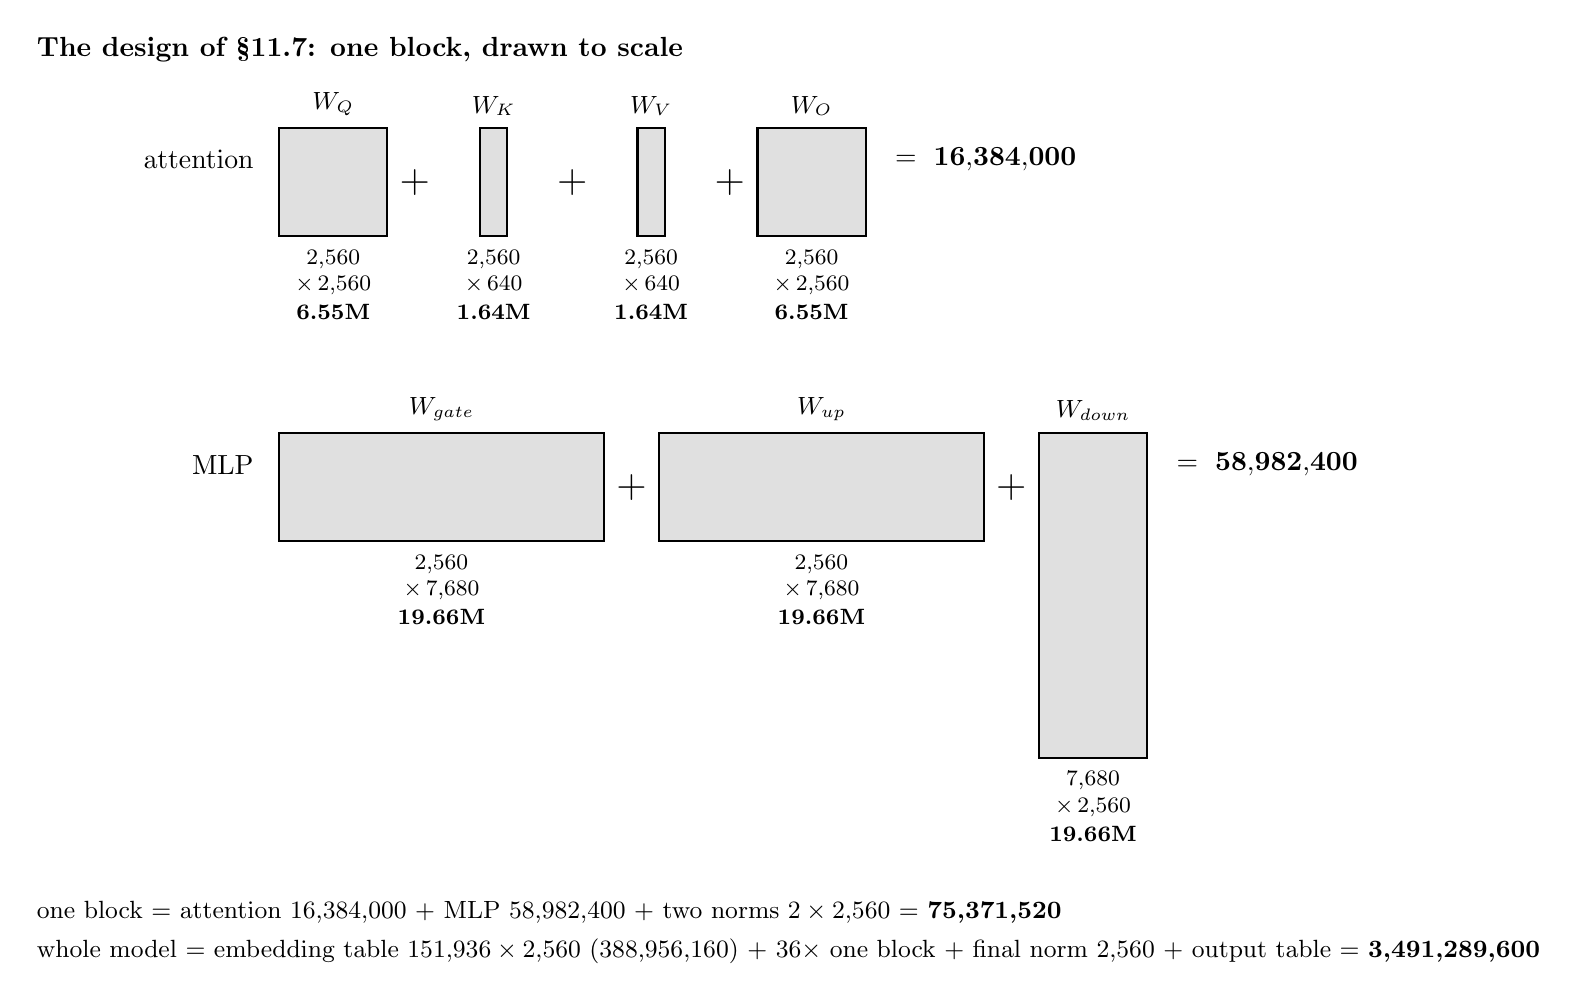
\begin{tikzpicture}
\node[anchor=west, font=\normalsize\bfseries] at (-3.2,1.0) {The design of \S11.7: one block, drawn to scale};
\node[anchor=east, font=\normalsize, align=right] at (-0.200,-0.400) {attention};
\draw[line width=0.8pt, fill=black!12] (0.000,0.000) rectangle (1.375,-1.375);
\node[anchor=south, font=\small] at (0.688,0.030) {$W_Q$};
\node[anchor=north, font=\footnotesize, align=center] at (0.688,-1.425) {2{,}560\\$\times$\,2{,}560\\[1pt]\textbf{6.55M}};
\node[font=\Large] at (1.725,-0.688) {$+$};
\draw[line width=0.8pt, fill=black!12] (2.553,0.000) rectangle (2.897,-1.375);
\node[anchor=south, font=\small] at (2.725,0.030) {$W_K$};
\node[anchor=north, font=\footnotesize, align=center] at (2.725,-1.425) {2{,}560\\$\times$\,640\\[1pt]\textbf{1.64M}};
\node[font=\Large] at (3.725,-0.688) {$+$};
\draw[line width=0.8pt, fill=black!12] (4.553,0.000) rectangle (4.897,-1.375);
\node[anchor=south, font=\small] at (4.725,0.030) {$W_V$};
\node[anchor=north, font=\footnotesize, align=center] at (4.725,-1.425) {2{,}560\\$\times$\,640\\[1pt]\textbf{1.64M}};
\node[font=\Large] at (5.725,-0.688) {$+$};
\draw[line width=0.8pt, fill=black!12] (6.075,0.000) rectangle (7.450,-1.375);
\node[anchor=south, font=\small] at (6.763,0.030) {$W_O$};
\node[anchor=north, font=\footnotesize, align=center] at (6.763,-1.425) {2{,}560\\$\times$\,2{,}560\\[1pt]\textbf{6.55M}};
\node[anchor=west, font=\normalsize] at (7.700,-0.400) {$=\ \mathbf{16{,}384{,}000}$};
\node[anchor=east, font=\normalsize, align=right] at (-0.200,-4.275) {MLP};
\draw[line width=0.8pt, fill=black!12] (0.000,-3.875) rectangle (4.125,-5.250);
\node[anchor=south, font=\small] at (2.062,-3.845) {$W_{\text{gate}}$};
\node[anchor=north, font=\footnotesize, align=center] at (2.062,-5.300) {2{,}560\\$\times$\,7{,}680\\[1pt]\textbf{19.66M}};
\node[font=\Large] at (4.475,-4.562) {$+$};
\draw[line width=0.8pt, fill=black!12] (4.825,-3.875) rectangle (8.950,-5.250);
\node[anchor=south, font=\small] at (6.888,-3.845) {$W_{\text{up}}$};
\node[anchor=north, font=\footnotesize, align=center] at (6.888,-5.300) {2{,}560\\$\times$\,7{,}680\\[1pt]\textbf{19.66M}};
\node[font=\Large] at (9.300,-4.562) {$+$};
\draw[line width=0.8pt, fill=black!12] (9.650,-3.875) rectangle (11.025,-8.000);
\node[anchor=south, font=\small] at (10.337,-3.845) {$W_{\text{down}}$};
\node[anchor=north, font=\footnotesize, align=center] at (10.337,-8.050) {7{,}680\\$\times$\,2{,}560\\[1pt]\textbf{19.66M}};
\node[anchor=west, font=\normalsize] at (11.275,-4.275) {$=\ \mathbf{58{,}982{,}400}$};
\node[anchor=north west, font=\small, align=left] at (-3.2,-9.700) {one block $=$ attention 16{,}384{,}000 $+$ MLP 58{,}982{,}400 $+$ two norms $2\times2{,}560$ $=$ \textbf{75{,}371{,}520}\\[3pt]whole model $=$ embedding table $151{,}936\times2{,}560$ (388{,}956{,}160) $+\ 36\times$ one block $+$ final norm 2{,}560 $+$ output table $=$ \textbf{3{,}491{,}289{,}600}};
\end{tikzpicture}}

\caption{One block of the \S11.7 design as a sum of its weight matrices, drawn to scale. The thin $W_K$ and
$W_V$ are the price of grouped-query attention paid in reverse: fewer key--value heads, fewer numbers to store.}
\end{figure}

\paragraph{Your turn, with fewer steps given.} Design for the phone of \S11.5: 4 GB in total, a
4{,}096-token context. Assume 4-bit weights and a 16-bit cache. Write down: the largest parameter count
that leaves 1 GB for the phone, a width and depth near it, and how many key--value heads you need. Use the
formulas of \S11.3 and \S11.5; Exercise 11.3 walks through one answer.

\begin{principle}{a design is a set of decisions with written-down assumptions}
Every line in the table has the same form: an assumption (``it will run with 8{,}192 tokens''), a
consequence you can compute (``\nElevenBKvGB\ GB of cache''), and a decision. The same form works for systems built
around models. In an agent's memory system, the context window is a budget measured in tokens, and every
token placed in it costs KV memory and attention time; deciding what to retrieve is deciding what is worth
that cost. The model does not make these decisions for you, and the arithmetic of this chapter is how you
make them in the open.
\end{principle}

%=====================================================================
\subsection*{11.8\quad The trade-off table}

\begin{center}
\small
\begin{tabular}{@{}P{3.2cm} P{5.4cm} P{5.4cm}@{}}
\toprule
Choice & What you gain & What you pay\\
\midrule
wider ($d$ up) & more numbers per token & parameters and FLOPs grow with $d^2$\\
deeper ($L$ up) & more steps of processing & time per token; harder to train without pre-norm\\
more heads, same $d$ & more kinds of question & less detail per question; no parameter change\\
fewer KV heads (GQA, MQA) & smaller KV cache, faster generation & a little flexibility; little measured loss\\
bigger vocabulary & shorter sequences & a bigger table and output layer\\
longer context & more text in view & KV memory and attention time grow with it\\
pre-norm vs post-norm & stable deep training & a slightly different signal path (Ch.\ 6)\\
RoPE vs learned positions & relative positions, longer contexts & nothing measurable in most reports\\
more training tokens & a better model at the same size & training compute ($6ND$)\\
\bottomrule
\end{tabular}
\end{center}

\Summary{Every choice in a transformer buys something specific and pays for it in compute, parameters,
memory or time, and you can write down which before you train.}

%=====================================================================
\begin{lookingback}
\begin{enumerate}[label=\arabic*.,leftmargin=1.6em]
\item (Chapter 3) Why do we divide attention scores by $\sqrt{d_k}$, and what would happen to a model with
$d_h=128$ if we did not?
\item (Chapter 9) Why does the KV cache store keys and values but not queries?
\item (Chapter 1) Which failure of the RNN does the ``time per token grows with depth'' cost in \S11.3
remind you of, and why is it less severe?
\end{enumerate}
\end{lookingback}

\subsection*{Exercises}

\begin{exercise}
A team has $C=6\times10^{20}$ FLOPs. Using the 20-tokens-per-parameter rule, find $N$ and $D$.
\end{exercise}

\begin{exercise}
Count the parameters inside one block of a model with $d=512$, $H=8$, $H_{kv}=2$, $d_h=64$ and a SwiGLU MLP
with $d_{ff}=1536$, ignoring the norm vectors. What share is attention?
\end{exercise}

\begin{exercise}
The phone of \S11.7: 4 GB in total, 1 GB kept for the phone, 4-bit weights, a 16-bit cache, 4{,}096
tokens. If you copy Qwen3-0.6B's attention shape ($L=28$, $d_h=128$, $H_{kv}=8$), how much is left for the
weights, and how many parameters is that?
\end{exercise}

\begin{exercise}
Your colleague trains one model with 8 heads and one with 2 heads and reports a validation loss of 1.41
versus 1.44. Write the two questions you would ask before believing that 8 heads are better.
\end{exercise}

\subsection*{Answers to Chapter 11}

\paragraph{Check yourself 11.1.} \emph{(c)}. With $C=6ND$ fixed, making $N$ four times bigger forces $D$
to a quarter, which moves you from 20 tokens per parameter to 1.25: far from the balance, so the plan is
wrong, not the arithmetic. (a) is M11.3: compute depends on tokens too. (b) is the correct arithmetic but
accepts the imbalance as if it were fine. (d) is M11.2: more data would need more compute than you have.

\paragraph{Check yourself 11.2.} \emph{(b)}. Every matrix has $d$ on at least one side, and most have it
on both (or $d$ and $d_{ff}=3d$), so the count grows about four times. (a) treats a matrix like a list.
(c) is M11.7, width as free. (d) mixes up the number of heads with their size; at fixed $d_h$ doubling $d$
doubles the heads.

\paragraph{Check yourself 11.3.} \emph{(b)}. The cache is proportional to $H_{kv}$ times the tokens, so
4 times the tokens and a quarter of the key--value heads cancel. (a) shrinks the weights, not the cache
(M11.4). (c) is M11.4 itself. (d) changes the queries, which are never cached (Chapter 9).

\paragraph{Exercise 11.1.} $N=\sqrt{C/120}=\sqrt{5\times10^{18}}\approx\nElevenExOneN$ parameters, and
$D=20N\approx\nElevenExOneD$ tokens. Check by putting both back into $6ND$: you get $6\times10^{20}$ again.

\paragraph{Exercise 11.2.} $W_Q$: $512\times512=\nElevenExTwoWq$; $W_K$ and $W_V$ together: $2\times512\times(2\times64)=\nElevenExTwoWkv$;
$W_O$: \nElevenExTwoWq; attention total \nElevenExTwoAttn. MLP: $3\times512\times1536=\nElevenExTwoMlp$. Block total
\nElevenExTwoBlock, of which attention is about \nElevenExTwoShare\%. The strategy that worked: count each matrix as inputs
times outputs, and write the shapes before multiplying.

\paragraph{Exercise 11.3.} Cache: $2\times28\times8\times128\times4096\times2$ bytes $\approx\nElevenExThreeKv$ GB.
Left for weights: $4-1-\nElevenExThreeKv\approx\nElevenExThreeLeft$ GB. At half a byte per parameter, that is about \nElevenExThreeN\ 
parameters, so memory is not the limit here; speed on a phone processor will be. A sensible answer stays
much smaller and spends the margin on a longer context.

\paragraph{Exercise 11.4.} (1) How large is the difference between two runs of the \emph{same} model with
different seeds? In our runs it was \nElevenSpread, larger than this gap. (2) Did both models get the same
data, steps and parameters? At fixed width they did have the same parameters (\S11.4), so if the gap is
real it comes from the shape of attention, not size.

\subsection*{What you now know}

\paragraph{From this chapter.}
\begin{itemize}
\item Training compute is about $6ND$; for a fixed budget the loss-optimal split is about 20 tokens per
parameter, and small models meant for heavy use are trained far beyond it.
\item A matrix costs inputs times outputs: width is quadratic, depth linear, and the vocabulary table can be
a quarter of a small model. Our calculator matches the real model classes exactly.
\item Heads at fixed width change the shape of attention, not its size; sharing keys and values saves the
memory that grows with every token.
\item Small experiments need a noise estimate before their results mean anything.
\end{itemize}

\paragraph{From the whole notes.} You started with one message, \tok{waste of time}, and a job: reply well.
\begin{itemize}
\item Writing is repeated next-word guessing, and the problem labels itself (Chapter 1).
\item Tokens become arrows, and similar tokens get nearby arrows (Chapter 2).
\item Attention lets each token ask, be found, and hand over, all at once for a whole batch (Chapter 3).
\item Rotating queries and keys gives order back (Chapter 4).
\item Heads, the MLP and the residual stream let tokens talk and then think (Chapter 5); normalisation lets
you stack many blocks (Chapter 6).
\item Scores become words through the output table, softmax and sampling (Chapter 7); training turns and
stretches the arrows (Chapter 8).
\item The KV cache makes generation fast and costs memory (Chapter 9); GPT-2 and Qwen3 are the same machine at
scale (Chapter 10).
\item And every number in a real model is a decision you can now price and defend (Chapter 11).
\end{itemize}
